\documentclass{article}

\usepackage{amsmath, amsthm, amssymb, amsfonts}
\usepackage{thmtools}
\usepackage{graphicx}
\usepackage{setspace}
\usepackage{geometry}
\usepackage{float}
\usepackage{hyperref}
\usepackage[utf8]{inputenc}
\usepackage{subfiles}
\usepackage[english]{babel}
\usepackage{framed}
\usepackage[dvipsnames]{xcolor}
\usepackage{tcolorbox}
% Added for topological diagrams
\usepackage{tikz}
\usetikzlibrary{topaths,calc}

% Color definitions
\colorlet{LightGray}{White!90!Periwinkle}
\colorlet{LightOrange}{Orange!15}
\colorlet{LightGreen}{Green!15}
\colorlet{LightBlue}{Cyan!15} % For Examples environment

% Rule command
\newcommand{\HRule}[1]{\rule{\linewidth}{#1}}

% Theorem styles
\declaretheoremstyle[name=Theorem,]{thmsty}
\declaretheorem[style=thmsty,numberwithin=section]{theorem}
\tcolorboxenvironment{theorem}{colback=LightGray}

\declaretheoremstyle[name=Proposition,]{prosty}
\declaretheorem[style=prosty,numberlike=theorem]{proposition}
\tcolorboxenvironment{proposition}{colback=LightOrange}

\declaretheoremstyle[name=Principle,]{prcpsty}
\declaretheorem[style=prcpsty,numberlike=theorem]{principle}
\tcolorboxenvironment{principle}{colback=LightGreen}

\declaretheoremstyle[name=Definition,]{defsty}
\declaretheorem[style=defsty,numberlike=theorem]{definition}
\tcolorboxenvironment{definition}{colback=white}

% New Examples environment
\declaretheoremstyle[name=Example,]{exsty}
\declaretheorem[style=exsty,numberlike=theorem]{example}
\tcolorboxenvironment{example}{colback=LightBlue}

\declaretheoremstyle[name=Corollary,]{corsty}
\declaretheorem[style=corsty,numberlike=theorem]{corollary}
\tcolorboxenvironment{corollary}{colback=LightGray}

% Document spacing and geometry
\setstretch{1.2}
\geometry{
    textheight=9in,
    textwidth=5.5in,
    top=1in,
    headheight=12pt,
    headsep=25pt,
    footskip=30pt
}

% Custom command for topology-specific notation
\newcommand{\topspace}[2]{\mathcal{#1}, \tau_{#2}} % e.g., \topspace{X}{1} for (X, τ_1)

\begin{document}

% Cover Page
\title{ \normalsize \textsc{Topology Notes}
\\ [2.0cm]
\HRule{1.5pt} \\
\LARGE \textbf{\uppercase{Introduction to Topology}
\HRule{2.0pt} \\ [0.6cm] \LARGE{Concepts and Examples} \vspace*{10\baselineskip}}
}
\date{\today}
\author{\textbf{Frank Yin} \\
	Self-learning Maths \\
	Sweden}

\maketitle
\newpage

\tableofcontents
\newpage

% Include chapters
\section{Introduction to Topology and Topological Spaces}

Topology is a field of mathematics that explores the properties of spaces preserved under continuous deformations—stretching, bending, or twisting, but not tearing or gluing. Often dubbed ``rubber-sheet geometry,'' it abstracts geometric notions like continuity, proximity, and connectivity into a general framework.

\subsection{Definition of a Topological Space}

\begin{definition}
A topological space is a pair $(X,\tau)$, where $X$ is a set and $\tau$ is a collection of subsets of $X$, called open sets, satisfying three axioms:
\begin{enumerate}
    \item \textbf{Inclusion of Extremes:} The empty set $\emptyset$ and the entire set $X$ are in $\tau$.
    \item \textbf{Closure under Arbitrary Unions:} If $\{U_\alpha\}_{\alpha \in A} \subseteq \tau$, then $\bigcup_{\alpha \in A} U_\alpha \in \tau$.
    \item \textbf{Closure under Finite Intersections:} If $U_1, U_2, \ldots, U_n \in \tau$, then $\bigcap_{i=1}^n U_i \in \tau$.
\end{enumerate}
The collection $\tau$ is called a topology on $X$.
\end{definition}

\begin{example}
Some fundamental examples of topological spaces:

\begin{enumerate}
    \item \textbf{Euclidean Space $\mathbb{R}^n$:} The standard topology is generated by open balls $B(x,r) = \{y \in \mathbb{R}^n \mid \|y-x\| < r\}$, where $\|\cdot\|$ is the Euclidean norm. The collection of all unions of such balls defines the topology.
    
    \item \textbf{Discrete Topology:} On any set $X$, take $\tau = \mathcal{P}(X)$, the power set. Every subset is open, making this the "finest" topology—points are as separated as possible.
    
    \item \textbf{Trivial (Indiscrete) Topology:} For any set $X$, $\tau = \{\emptyset, X\}$. Only the extremes are open, the "coarsest" topology, where distinguishing points is impossible.
    
    \item \textbf{Cofinite Topology:} On an infinite set $X$, $\tau = \{U \subseteq X \mid X \setminus U \text{ is finite}\} \cup \{\emptyset\}$. Open sets are those with finite complements.
    
    \item \textbf{Subspace Topology:} Given $(X,\tau)$ and $Y \subseteq X$, the topology on $Y$ is $\tau_Y = \{U \cap Y \mid U \in \tau\}$. For example, the interval $[0,1]$ inherits its topology from $\mathbb{R}$.
\end{enumerate}
\end{example}

\subsection{Basis for a Topology}

\begin{definition}
A basis $\mathcal{B} \subseteq \tau$ generates the topology if every open set in $\tau$ is a union of sets from $\mathcal{B}$. 
\end{definition}

\begin{example}
For $\mathbb{R}$, the collection of open intervals $(a,b)$ forms a basis for the standard topology.
\end{example}

\begin{figure}[h]
\centering
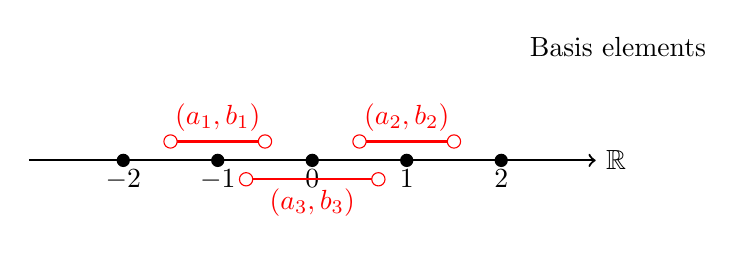
\begin{tikzpicture}[scale=1.2]
    % Drawing the real line
    \draw[->,thick] (-3,0) -- (3,0) node[right] {$\mathbb{R}$};
    
    % Marking some points
    \foreach \x in {-2,-1,0,1,2} {
        \fill (\x,0) circle (2pt);
        \node[below] at (\x,0) {$\x$};
    }
    
    % Drawing open intervals as basis elements
    \draw[red, thick] (-1.5,0.2) -- (-0.5,0.2);
    \draw[red, thick] (0.5,0.2) -- (1.5,0.2);
    \draw[red, thick] (-0.7,-0.2) -- (0.7,-0.2);
    
    % Endpoints
    \draw[red, fill=white] (-1.5,0.2) circle (2pt);
    \draw[red, fill=white] (-0.5,0.2) circle (2pt);
    \draw[red, fill=white] (0.5,0.2) circle (2pt);
    \draw[red, fill=white] (1.5,0.2) circle (2pt);
    \draw[red, fill=white] (-0.7,-0.2) circle (2pt);
    \draw[red, fill=white] (0.7,-0.2) circle (2pt);
    
    % Labels
    \node[red, above] at (-1,0.2) {$(a_1,b_1)$};
    \node[red, above] at (1,0.2) {$(a_2,b_2)$};
    \node[red, below] at (0,-0.2) {$(a_3,b_3)$};
    
    \node[above right] at (2.2,1) {Basis elements};
\end{tikzpicture}
\caption{Open intervals as basis elements for $\mathbb{R}$ with standard topology}
\end{figure}

\subsection{Motivation and Intuition}

Topology generalizes the notion of "nearness" without requiring a metric. The axioms ensure a structure flexible enough to study continuity abstractly, yet robust enough to classify spaces.

\section{Basic Topological Properties}

These properties form the building blocks for understanding how topological spaces behave.

\subsection{Open and Closed Sets}

\begin{definition}
In a topological space $(X, \tau)$:
\begin{itemize}
    \item \textbf{Open Sets:} Defined by the topology $\tau$.
    \item \textbf{Closed Sets:} A set $A \subseteq X$ is closed if its complement $X \setminus A$ is open.
\end{itemize}
\end{definition}

\begin{proposition}
Properties of closed sets:
\begin{enumerate}
    \item $\emptyset$ and $X$ are closed (complements of $X$ and $\emptyset$).
    \item Arbitrary intersections of closed sets are closed.
    \item Finite unions of closed sets are closed.
\end{enumerate}
\end{proposition}

\begin{example}
In $\mathbb{R}$ with the standard topology:
\begin{itemize}
    \item $(0,1)$ is open.
    \item $[0,1]$ is closed, since $\mathbb{R} \setminus [0,1] = (-\infty,0) \cup (1,\infty)$ is open.
    \item $(0,1]$ is neither open nor closed, as $(0,1]$ excludes $0$ (not open) and $\mathbb{R} \setminus (0,1] = (-\infty,0] \cup (1,\infty)$ isn't open.
\end{itemize}
\end{example}

\begin{figure}[h]
\centering
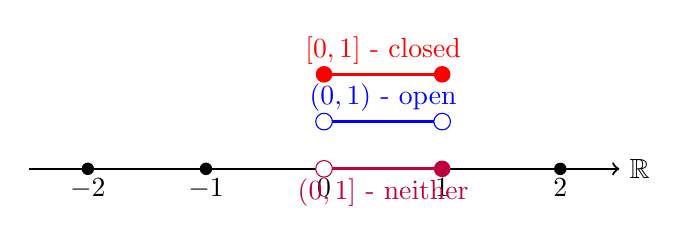
\begin{tikzpicture}[scale=1.5]
    % Drawing the real line
    \draw[->,thick] (-2.5,0) -- (2.5,0) node[right] {$\mathbb{R}$};
    
    % Marking some points
    \foreach \x in {-2,-1,0,1,2} {
        \fill (\x,0) circle (1.5pt);
        \node[below] at (\x,0) {$\x$};
    }
    
    % Drawing intervals with different topological properties
    \draw[blue, very thick] (0,0.4) -- (1,0.4);
    \draw[blue, fill=white] (0,0.4) circle (2pt);
    \draw[blue, fill=white] (1,0.4) circle (2pt);
    \node[blue, above] at (0.5,0.4) {$(0,1)$ - open};
    
    \draw[red, very thick] (0,0.8) -- (1,0.8);
    \fill[red] (0,0.8) circle (2pt);
    \fill[red] (1,0.8) circle (2pt);
    \node[red, above] at (0.5,0.8) {$[0,1]$ - closed};
    
    \draw[purple, very thick] (0,0) -- (1,0);
    \draw[purple, fill=white] (0,0) circle (2pt);
    \fill[purple] (1,0) circle (2pt);
    \node[purple, below] at (0.5,0) {$(0,1]$ - neither};
\end{tikzpicture}
\caption{Different types of sets in $\mathbb{R}$}
\end{figure}

\subsection{Compactness}

\begin{definition}
A space $X$ is compact if every open cover has a finite subcover. An open cover is a collection $\{U_\alpha\}_{\alpha \in A} \subseteq \tau$ such that $X = \bigcup_{\alpha \in A} U_\alpha$. A finite subcover is a finite subset $\{U_{\alpha_1}, \ldots, U_{\alpha_n}\}$ with $X = \bigcup_{i=1}^n U_{\alpha_i}$.
\end{definition}

\begin{theorem}[Heine-Borel Theorem]
In $\mathbb{R}^n$, a subset is compact if and only if it is closed and bounded.
\end{theorem}

\begin{example}
\begin{enumerate}
    \item $[0,1]$ is compact in $\mathbb{R}$. The cover $\{(1/n,1] \mid n=2,3,\ldots\} \cup \{(0,1/2)\}$ reduces to $(0,1/2)$ and $(1/2,1]$.
    
    \item $(0,1)$ is not compact. The cover $\{(1/n,1-1/n) \mid n=2,3,\ldots\}$ has no finite subcover, as it misses points near 0 and 1.
\end{enumerate}
\end{example}

\begin{figure}[h]
\centering
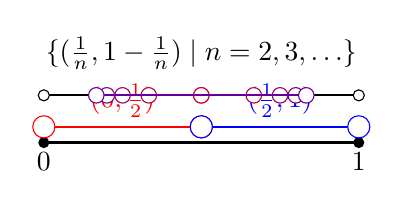
\begin{tikzpicture}[scale=4]
    % Drawing the interval [0,1]
    \draw[thick] (0,0) -- (1,0);
    \fill (0,0) circle (0.5pt);
    \fill (1,0) circle (0.5pt);
    \node[below] at (0,0) {$0$};
    \node[below] at (1,0) {$1$};
    
    % Showing a finite subcover for [0,1]
    \draw[red, thick] (0,0.05) -- (0.5,0.05);
    \draw[blue, thick] (0.5,0.05) -- (1,0.05);
    \draw[red, fill=white] (0,0.05) circle (1pt);
    \draw[red, fill=white] (0.5,0.05) circle (1pt);
    \draw[blue, fill=white] (0.5,0.05) circle (1pt);
    \draw[blue, fill=white] (1,0.05) circle (1pt);
    
    \node[red, above] at (0.25,0.05) {$(0,\frac{1}{2})$};
    \node[blue, above] at (0.75,0.05) {$(\frac{1}{2},1)$};
    
    % Showing a cover with no finite subcover for (0,1)
    \draw[thick] (0,0.15) -- (1,0.15);
    \draw[fill=white] (0,0.15) circle (0.5pt);
    \draw[fill=white] (1,0.15) circle (0.5pt);
    
    \foreach \n in {2,3,4,5,6} {
        \pgfmathsetmacro{\start}{1/\n}
        \pgfmathsetmacro{\end}{1-1/\n}
        \colorlet{mycolor\n}{blue!\n0!red}
        \draw[mycolor\n, thick] (\start,0.15) -- (\end,0.15);
        \draw[mycolor\n, fill=white] (\start,0.15) circle (0.7pt);
        \draw[mycolor\n, fill=white] (\end,0.15) circle (0.7pt);
    }
    
    \node[above] at (0.5,0.2) {$\{(\frac{1}{n},1-\frac{1}{n}) \mid n=2,3,\ldots\}$};
\end{tikzpicture}
\caption{Compactness illustrated on intervals in $\mathbb{R}$}
\end{figure}

\subsection{Connectedness}

\begin{definition}
A space $X$ is connected if it cannot be written as $X = U \cup V$, where $U$ and $V$ are disjoint, non-empty open sets. Equivalently, the only subsets that are both open and closed (clopen) are $\emptyset$ and $X$.
\end{definition}

\begin{definition}
A space $X$ is path-connected if any two points can be joined by a continuous path $\gamma: [0,1] \to X$. Path-connected implies connected, but not vice versa.
\end{definition}

\begin{example}
\begin{enumerate}
    \item $\mathbb{R}$ is connected. Suppose $\mathbb{R} = U \cup V$, $U \cap V = \emptyset$, both open and non-empty. By the intermediate value theorem, a continuous function separating $U$ and $V$ leads to a contradiction.
    
    \item $\{0\} \cup \{1\} \subset \mathbb{R}$ is not connected, as $\{0\} = (-\infty,1/2) \cap \{0,1\}$ and $\{1\} = (1/2,\infty) \cap \{0,1\}$ are open in the subspace topology.
\end{enumerate}
\end{example}

\begin{figure}[h]
\centering
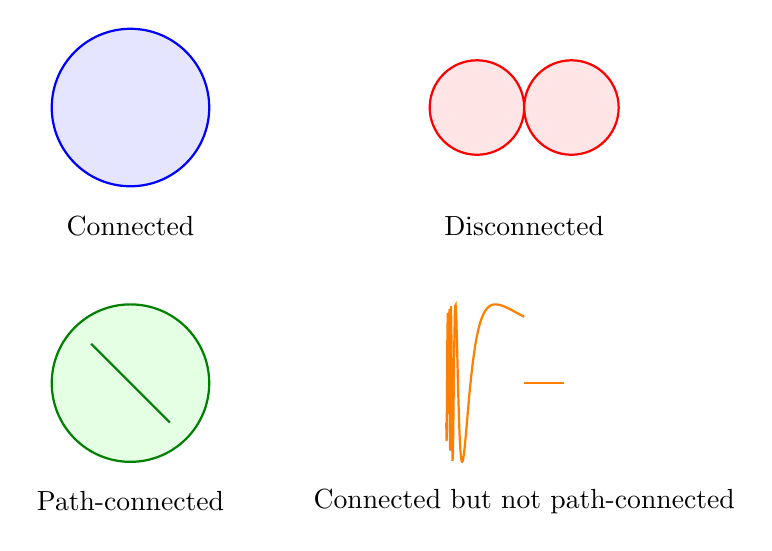
\begin{tikzpicture}
    % Connected space example - Circle
    \begin{scope}[shift={(-2.5,0)}]
        \draw[thick, blue, fill=blue!10] (0,0) circle (1);
        \node at (0,-1.5) {Connected};
    \end{scope}
    
    % Disconnected space example - Two circles
    \begin{scope}[shift={(2.5,0)}]
        \draw[thick, red, fill=red!10] (-0.6,0) circle (0.6);
        \draw[thick, red, fill=red!10] (0.6,0) circle (0.6);
        \node at (0,-1.5) {Disconnected};
    \end{scope}
    
    % Path-connected example
    \begin{scope}[shift={(-2.5,-3.5)}]
        \draw[thick, green!50!black, fill=green!10] (0,0) circle (1);
        \draw[thick, green!50!black] (-0.5,0.5) -- (0.5,-0.5);
        \node at (0,-1.5) {Path-connected};
    \end{scope}
    
    % Connected but not path-connected example (topologist's sine curve)
    \begin{scope}[shift={(2.5,-3.5)}]
        \draw[thick, orange] plot[domain=-0.99:0, samples=200] (\x, {sin(1/(\x+1) r)});
        \draw[thick, orange] (0,0) -- (0.5,0);
        \node at (0,-1.5) {Connected but not path-connected};
    \end{scope}
\end{tikzpicture}
\caption{Different types of connectedness in topological spaces}
\end{figure}

\section{Continuous Deformations and Homeomorphisms}

\subsection{Continuous Functions}

\begin{definition}
A function $f: X \to Y$ between topological spaces is continuous if for every open set $V \subseteq Y$, the preimage $f^{-1}(V)$ is open in $X$. This generalizes the $\epsilon$-$\delta$ definition from metric spaces.
\end{definition}

\begin{example}
$f: \mathbb{R} \to \mathbb{R}$, $f(x) = x^2$, is continuous, as preimages of open intervals are open (e.g., $f^{-1}((1,4)) = (-2,-1) \cup (1,2)$).
\end{example}

\begin{figure}[h]
\centering
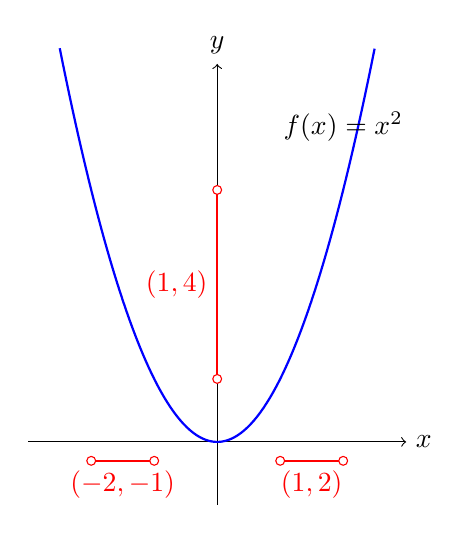
\begin{tikzpicture}[scale=0.8]
    % Drawing axes for domain
    \draw[->] (-3,0) -- (3,0) node[right] {$x$};
    \draw[->] (0,-1) -- (0,6) node[above] {$y$};
    
    % Drawing the parabola
    \draw[thick, blue, domain=-2.5:2.5, samples=100] plot (\x, {(\x)^2});
    
    % Marking the interval (1,4) on the y-axis
    \draw[red, thick] (0,1) -- (0,4);
    \draw[red, fill=white] (0,1) circle (2pt);
    \draw[red, fill=white] (0,4) circle (2pt);
    \node[red, left] at (0,2.5) {$(1,4)$};
    
    % Marking the preimage on the x-axis
    \draw[red, thick] (-2,-0.3) -- (-1,-0.3);
    \draw[red, thick] (1,-0.3) -- (2,-0.3);
    \draw[red, fill=white] (-2,-0.3) circle (2pt);
    \draw[red, fill=white] (-1,-0.3) circle (2pt);
    \draw[red, fill=white] (1,-0.3) circle (2pt);
    \draw[red, fill=white] (2,-0.3) circle (2pt);
    \node[red, below] at (-1.5,-0.3) {$(-2,-1)$};
    \node[red, below] at (1.5,-0.3) {$(1,2)$};
    
    % Label
    \node at (2,5) {$f(x) = x^2$};
\end{tikzpicture}
\caption{Continuity of $f(x) = x^2$ illustrated by preimages}
\end{figure}

\subsection{Homeomorphisms}

\begin{definition}
A homeomorphism is a bijective continuous function $f: X \to Y$ with a continuous inverse $f^{-1}: Y \to X$. Spaces $X$ and $Y$ are homeomorphic ($X \cong Y$) if such an $f$ exists—they are topologically identical.
\end{definition}

\begin{example}
\begin{enumerate}
    \item $(0,1) \cong \mathbb{R}$ via $f(x) = \tan(\pi x - \pi/2)$, with inverse $f^{-1}(y) = \frac{\arctan(y)}{\pi} + \frac{1}{2}$, both continuous.
    
    \item A sphere $S^2$ and an ellipsoid are homeomorphic—deform one into the other smoothly.
    
    \item $S^2$ and a torus $T^2$ are not homeomorphic due to differing hole structures.
\end{enumerate}
\end{example}

\begin{example}[Counterexample]
The circle $S^1$ and the interval $[0,1]$ are not homeomorphic. Removing a point from $S^1$ leaves it connected, while removing an interior point from $[0,1]$ disconnects it.
\end{example}

\begin{figure}[h]
\centering
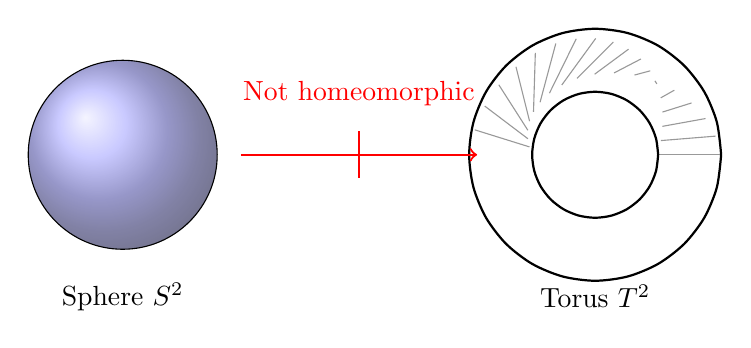
\begin{tikzpicture}
    % Drawing a sphere
    \begin{scope}[shift={(-3,0)}]
        \shade[ball color=blue!40, opacity=0.7] (0,0) circle (1.2);
        \draw (0,0) circle (1.2);
        \node at (0,-1.8) {Sphere $S^2$};
    \end{scope}
    
    % Drawing a torus
    \begin{scope}[shift={(3,0)}]
        \pgfmathsetmacro{\R}{1.2}
        \pgfmathsetmacro{\r}{0.4}
        
        \foreach \t in {0,10,...,350} {
            \draw[black!70] ({(\R+\r*cos(\t))*cos(\t)},{(\R+\r*cos(\t))*sin(\t)},{1.5*\r*sin(\t)});
        }
        
        \foreach \t in {0,10,...,170} {
            \pgfmathsetmacro{\angle}{\t}
            \pgfmathsetmacro{\opangle}{180+\t}
            \draw[black!40] ({(\R+\r*cos(\angle))*cos(\t)},{(\R+\r*cos(\angle))*sin(\t)},{1.5*\r*sin(\angle)}) -- ({(\R+\r*cos(\opangle))*cos(\t)},{(\R+\r*cos(\opangle))*sin(\t)},{1.5*\r*sin(\opangle)});
        }
        
        \draw[thick] plot[domain=0:360,smooth,variable=\t] ({(\R+\r)*cos(\t)},{(\R+\r)*sin(\t)},0);
        \draw[thick] plot[domain=0:360,smooth,variable=\t] ({(\R-\r)*cos(\t)},{(\R-\r)*sin(\t)},0);
        
        \node at (0,-1.8) {Torus $T^2$};
    \end{scope}
    
    % Non-homeomorphic indication
    \draw[thick, red, ->] (-1.5,0) -- (1.5,0);
    \draw[thick, red] (0,0.3) -- (0,-0.3);
    \node[red, above] at (0,0.5) {Not homeomorphic};
\end{tikzpicture}
\caption{Sphere and torus are not homeomorphic}
\end{figure}

\subsection{Topological Invariants}

\begin{definition}
A topological invariant is a property that is preserved under homeomorphisms.
\end{definition}

\begin{proposition}
Properties invariant under homeomorphisms include:
\begin{itemize}
    \item Connectedness
    \item Compactness
    \item Number of connected components
    \item Euler characteristic
\end{itemize}
\end{proposition}

\section{Homology: Understanding Holes}

Homology is an algebraic tool in topology that quantifies "holes" in a space across dimensions, assigning abelian groups $H_n(X)$ to capture structural features.

\subsection{Intuition}

\begin{proposition}
Homology groups capture different types of "holes":
\begin{itemize}
    \item $H_0$: Counts connected components (0D holes).
    \item $H_1$: Counts loops or 1D holes.
    \item $H_2$: Counts voids or 2D holes.
\end{itemize}
\end{proposition}

\begin{example}
Visual examples:
\begin{itemize}
    \item Sphere $S^2$: One piece, no loops, one void.
    \item Torus $T^2$: One piece, two independent loops, one void.
\end{itemize}
\end{example}

\begin{figure}[h]
\centering
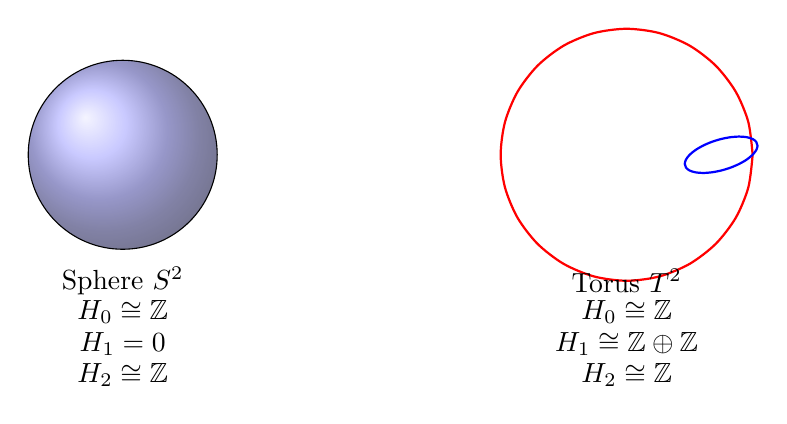
\begin{tikzpicture}[scale=0.8]
    % Sphere homology
    \begin{scope}[shift={(-4,0)}]
        \shade[ball color=blue!40, opacity=0.7] (0,0) circle (1.5);
        \draw (0,0) circle (1.5);
        \node at (0,-2) {Sphere $S^2$};
        \node at (0,-2.5) {$H_0 \cong \mathbb{Z}$};
        \node at (0,-3) {$H_1 = 0$};
        \node at (0,-3.5) {$H_2 \cong \mathbb{Z}$};
    \end{scope}
    
    % Torus homology
    \begin{scope}[shift={(4,0)}]
        \pgfmathsetmacro{\R}{1.5}
        \pgfmathsetmacro{\r}{0.5}
        
        \foreach \t in {0,10,...,350} {
            \draw[black!70] ({(\R+\r*cos(\t))*cos(\t)},{(\R+\r*cos(\t))*sin(\t)},{1.5*\r*sin(\t)});
        }
        
        % Draw meridional loop in red
        \draw[thick, red] plot[domain=0:360,smooth,variable=\t] ({(\R+\r*cos(0))*cos(\t)},{(\R+\r*cos(0))*sin(\t)},{1.5*\r*sin(0)}); 
        
        % Draw longitudinal loop in blue
        \draw[thick, blue] plot[domain=0:360,smooth,variable=\t] ({(\R+\r*cos(\t))},0,{1.5*\r*sin(\t)});
        
        \node at (0,-2) {Torus $T^2$};
        \node at (0,-2.5) {$H_0 \cong \mathbb{Z}$};
        \node at (0,-3) {$H_1 \cong \mathbb{Z} \oplus \mathbb{Z}$};
        \node at (0,-3.5) {$H_2 \cong \mathbb{Z}$};
    \end{scope}
\end{tikzpicture}
\caption{Homology groups of sphere and torus}
\end{figure}

\subsection{Simplicial Complexes}

\begin{definition}
A simplicial complex $K$ is a set of simplices such that:
\begin{enumerate}
    \item Every face of a simplex in $K$ is in $K$.
    \item The intersection of two simplices is either empty or a common face.
\end{enumerate}
\end{definition}

\begin{example}
Examples of simplicial complexes:
\begin{itemize}
    \item A triangle with vertices $\{v_0, v_1, v_2\}$, edges $\{[v_0, v_1], [v_1, v_2], [v_0, v_2]\}$, and face $[v_0, v_1, v_2]$.
    \item A tetrahedron, including all faces, edges, and vertices.
    \item A triangulation of $S^2$ as a mesh of triangles.
\end{itemize}
\end{example}

\begin{figure}[h]
\centering
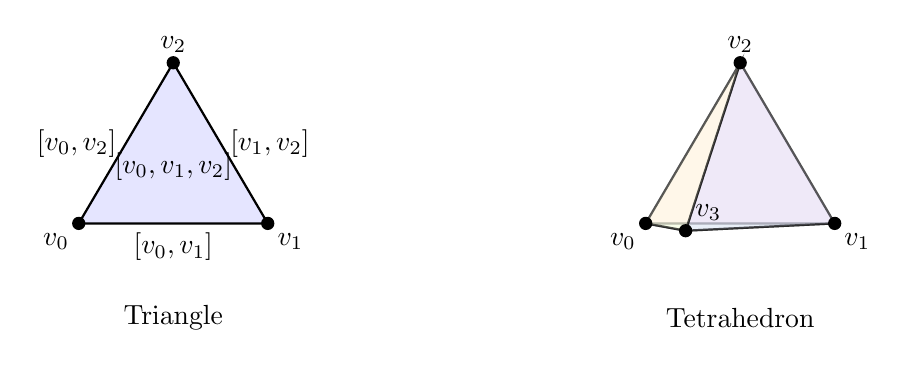
\begin{tikzpicture}[scale=1.2]
    % Triangle example
    \begin{scope}[shift={(-3,0)}]
        % Draw the triangle
        \draw[thick, fill=blue!10] (0,0) -- (2,0) -- (1,1.7) -- cycle;
        
        % Label vertices
        \fill (0,0) circle (2pt) node[below left] {$v_0$};
        \fill (2,0) circle (2pt) node[below right] {$v_1$};
        \fill (1,1.7) circle (2pt) node[above] {$v_2$};
        
        % Label edges
        \node[below] at (1,0) {$[v_0,v_1]$};
        \node[right] at (1.5,0.85) {$[v_1,v_2]$};
        \node[left] at (0.5,0.85) {$[v_0,v_2]$};
        
        % Label the face
        \node at (1,0.6) {$[v_0,v_1,v_2]$};
        
        \node at (1,-1) {Triangle};
    \end{scope}
    
    % Tetrahedron example
    \begin{scope}[shift={(3,0)}]
        % Draw the tetrahedron
        \coordinate (v0) at (0,0,0);
        \coordinate (v1) at (2,0,0);
        \coordinate (v2) at (1,1.7,0);
        \coordinate (v3) at (1,0.5,1.5);
        
        % Back face
        \draw[thick, black!30, fill=red!10, opacity=0.6] (v0) -- (v1) -- (v2) -- cycle;
        % Side faces
        \draw[thick, fill=green!10, opacity=0.6] (v0) -- (v1) -- (v3) -- cycle;
        \draw[thick, fill=blue!10, opacity=0.6] (v1) -- (v2) -- (v3) -- cycle;
        \draw[thick, fill=yellow!10, opacity=0.6] (v0) -- (v2) -- (v3) -- cycle;
        
        % Vertices
        \fill (v0) circle (2pt) node[below left] {$v_0$};
        \fill (v1) circle (2pt) node[below right] {$v_1$};
        \fill (v2) circle (2pt) node[above] {$v_2$};
        \fill (v3) circle (2pt) node[above right] {$v_3$};
        
        \node at (1,-1) {Tetrahedron};
    \end{scope}
\end{tikzpicture}
\caption{Examples of simplicial complexes}
\end{figure}

\subsection{Chains and Chain Groups}

\begin{definition}
For a simplicial complex $K$, the $n$-chain group $C_n(K)$ is the free abelian group generated by oriented $n$-simplices, with integer coefficients:
\begin{itemize}
    \item $C_0(K)$: Sums of vertices, e.g., $3v_1 - 2v_2$.
    \item $C_1(K)$: Sums of edges, e.g., $2[v_0, v_1] + [v_1, v_2]$.
    \item $C_2(K)$: Sums of triangles, e.g., $[v_0, v_1, v_2] - 2[v_1, v_2, v_3]$.
\end{itemize}
\end{definition}

\subsection{Boundary Operator}

\begin{definition}
The boundary operator $\partial_n: C_n(K) \to C_{n-1}(K)$ assigns to each $n$-simplex its oriented boundary:
\begin{itemize}
    \item $\partial_0(v) = 0$ (vertices have no boundary).
    \item $\partial_1([v_0, v_1]) = v_1 - v_0$ (end minus start).
    \item $\partial_2([v_0, v_1, v_2]) = [v_1, v_2] - [v_0, v_2] + [v_0, v_1]$ (edges in cyclic order, with signs reflecting orientation).
\end{itemize}
\end{definition}

\begin{theorem}
Fundamental Property: $\partial_{n-1} \circ \partial_n = 0$. The boundary of a boundary is zero.
\end{theorem}

\begin{example}
Verification of $\partial_1(\partial_2([v_0,v_1,v_2])) = 0$:
\begin{align*}
\partial_1(\partial_2([v_0,v_1,v_2])) &= \partial_1([v_1,v_2] - [v_0,v_2] + [v_0,v_1]) \\
&= (v_2 - v_1) - (v_2 - v_0) + (v_1 - v_0) \\
&= 0
\end{align*}
\end{example}

\begin{figure}[h]
\centering
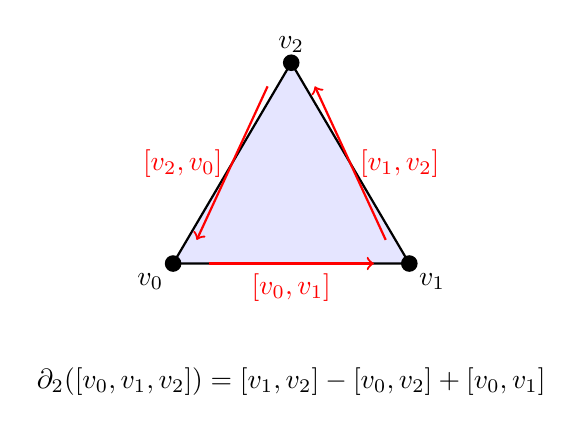
\begin{tikzpicture}[scale=1.5]
    % Draw a triangle
    \draw[thick, fill=blue!10] (0,0) -- (2,0) -- (1,1.7) -- cycle;
    
    % Label vertices
    \fill (0,0) circle (2pt) node[below left] {$v_0$};
    \fill (2,0) circle (2pt) node[below right] {$v_1$};
    \fill (1,1.7) circle (2pt) node[above] {$v_2$};
    
    % Label edges with orientations
    \draw[->, thick, red] (0.3,0) -- (1.7,0);
    \node[red, below] at (1,0) {$[v_0,v_1]$};
    
    \draw[->, thick, red] (1.8,0.2) -- (1.2,1.5);
    \node[red, right] at (1.5,0.85) {$[v_1,v_2]$};
    
    \draw[->, thick, red] (0.8,1.5) -- (0.2,0.2);
    \node[red, left] at (0.5,0.85) {$[v_2,v_0]$};
    
    % Boundary equation
    \node at (1,-1) {$\partial_2([v_0,v_1,v_2]) = [v_1,v_2] - [v_0,v_2] + [v_0,v_1]$};
\end{tikzpicture}
\caption{Boundary operator applied to a 2-simplex}
\end{figure}

\subsection{Cycles and Boundaries}

\begin{definition}
In a chain complex:
\begin{itemize}
    \item \textbf{Cycles:} $Z_n(K) = \ker \partial_n = \{ c \in C_n(K) \mid \partial_n c = 0 \}$, chains with no boundary (closed loops or surfaces).
    \item \textbf{Boundaries:} $B_n(K) = \operatorname{im} \partial_{n+1} = \{ c \in C_n(K) \mid c = \partial_{n+1} d, d \in C_{n+1}(K) \}$, chains that bound higher simplices.
\end{itemize}
Since $\partial_{n-1} \circ \partial_n = 0$, we have $B_n(K) \subseteq Z_n(K)$.
\end{definition}

\subsection{Homology Groups}

\begin{definition}
The $n$-th homology group is:
\begin{equation}
H_n(K) = Z_n(K) / B_n(K) = \frac{\ker \partial_n}{\operatorname{im} \partial_{n+1}}
\end{equation}
\end{definition}

\begin{proposition}
Interpretation: $H_n(K)$ consists of cycles not bounding anything, representing $n$-dimensional holes.
\end{proposition}

\begin{definition}
Rank: The free part's rank (Betti number $\beta_n$) counts independent $n$-holes; torsion captures twisting (rare in simple spaces).
\end{definition}

\begin{example}
Examples of homology computations:
\begin{enumerate}
    \item Sphere $S^2$ (triangulated):
    \begin{itemize}
        \item $H_0(S^2) \cong \mathbb{Z}$ (one connected component).
        \item $H_1(S^2) = 0$ (every 1-cycle bounds a 2-simplex; no loops).
        \item $H_2(S^2) \cong \mathbb{Z}$ (the surface encloses one void).
    \end{itemize}
    
    \item Torus $T^2$:
    \begin{itemize}
        \item $H_0(T^2) \cong \mathbb{Z}$ (one piece).
        \item $H_1(T^2) \cong \mathbb{Z} \oplus \mathbb{Z}$ (two loops: meridional and longitudinal).
        \item $H_2(T^2) \cong \mathbb{Z}$ (one enclosed void).
    \end{itemize}
    
    \item Figure-Eight (wedge of two circles):
    \begin{itemize}
        \item $H_0 \cong \mathbb{Z}$ (one component).
        \item $H_1 \cong \mathbb{Z} \oplus \mathbb{Z}$ (two distinct loops meeting at a point).
    \end{itemize}
\end{enumerate}
\end{example}

\begin{example}[Computation Example: Triangle with Interior]
Consider a filled triangle (a 2-simplex):
\begin{itemize}
    \item $C_0 = \langle v_0, v_1, v_2 \rangle \cong \mathbb{Z}^3$
    \item $C_1 = \langle [v_0, v_1], [v_1, v_2], [v_0, v_2] \rangle \cong \mathbb{Z}^3$
    \item $C_2 = \langle [v_0, v_1, v_2] \rangle \cong \mathbb{Z}$
    \item $\partial_2([v_0, v_1, v_2]) = [v_1, v_2] - [v_0, v_2] + [v_0, v_1]$
\end{itemize}

Homology groups:
\begin{itemize}
    \item $H_0 \cong \mathbb{Z}$ (connected).
    \item $H_1 = 0$ (the boundary cycle is $\partial_2$, so $Z_1 = B_1$).
    \item $H_2 = 0$ (the triangle is filled, so there is no 2-cycle that isn't a boundary).
\end{itemize}
\end{example}

\section{Euler Characteristic and Homology}

\begin{definition}
The Euler characteristic $\chi(K)$ links homology to combinatorics:
\begin{equation}
\chi(K) = \sum_{n=0}^\infty (-1)^n \operatorname{rank} H_n(K)
\end{equation}
Alternatively, for a simplicial complex: $\chi = V - E + F$ (vertices, edges, faces).
\end{definition}

\begin{example}
Examples of Euler characteristic calculations:
\begin{itemize}
    \item Sphere: $H_0 = \mathbb{Z}$, $H_1 = 0$, $H_2 = \mathbb{Z}$, so $\chi = 1 - 0 + 1 = 2$.
    \item Torus: $H_0 = \mathbb{Z}$, $H_1 = \mathbb{Z}^2$, $H_2 = \mathbb{Z}$, so $\chi = 1 - 2 + 1 = 0$.
\end{itemize}
\end{example}

\begin{theorem}
The Euler characteristic is a topological invariant, often related to genus $g$ (number of handles) by $\chi = 2 - 2g$ for closed surfaces.
\end{theorem}

\begin{figure}[h]
\centering
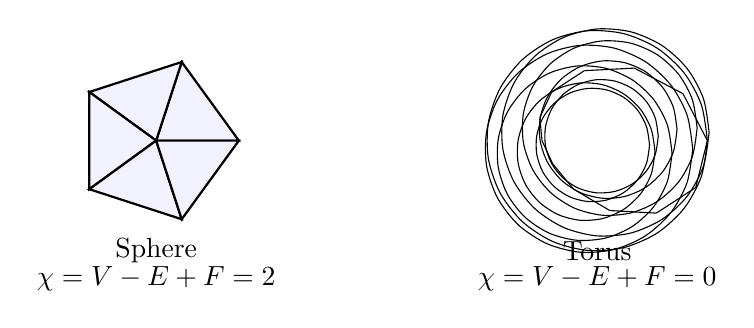
\begin{tikzpicture}[scale=0.7]
    % Triangulated sphere
    \begin{scope}[shift={(-4,0)}]
        % Draw an icosahedron as an approximation to a sphere
        \foreach \ang in {0,72,...,359} {
            \draw[thick, fill=blue!5] (0,0) -- ({1.5*cos(\ang)},{1.5*sin(\ang)}) -- ({1.5*cos(\ang+72)},{1.5*sin(\ang+72)}) -- cycle;
        }
        
        \node at (0,-2) {Sphere};
        \node at (0,-2.5) {$\chi = V - E + F = 2$};
    \end{scope}
    
    % Triangulated torus
    \begin{scope}[shift={(4,0)}]
        % Draw a simplified triangulated torus representation
        \pgfmathsetmacro{\R}{1.5}
        \pgfmathsetmacro{\r}{0.5}
        
        % Draw a simplified mesh on the surface
        \foreach \t in {0,30,...,330} {
            \draw[thin] ({(\R+\r*cos(\t))*cos(\t)},{(\R+\r*cos(\t))*sin(\t)},{1.2*\r*sin(\t)}) -- 
                        ({(\R+\r*cos(\t+30))*cos(\t+30)},{(\R+\r*cos(\t+30))*sin(\t+30)},{1.2*\r*sin(\t+30)});
        }
        
        \foreach \t in {0,40,...,320} {
            \draw[thin] plot[domain=0:360,smooth,variable=\s,samples=20] 
                ({(\R+\r*cos(\t))*cos(\s)},{(\R+\r*cos(\t))*sin(\s)},{1.2*\r*sin(\t)});
        }
        
        \node at (0,-2) {Torus};
        \node at (0,-2.5) {$\chi = V - E + F = 0$};
    \end{scope}
\end{tikzpicture}
\caption{Euler characteristic for sphere and torus}
\end{figure}


% References
\bibliographystyle{IEEEtran}
\begin{thebibliography}{1}
	\bibitem{Munkres}
	J. R. Munkres, \emph{Topology}, 2nd ed. Upper Saddle River, NJ: Prentice Hall, 2000.
\end{thebibliography}

\end{document}
